\documentclass{article}
\usepackage{hyperref}
\usepackage{amsmath}
\usepackage{amssymb}
\usepackage{pgfplots}
\usepackage{float}
\usepackage{todonotes}
\usepackage{tikz}
\usepackage[shortlabels]{enumitem}

\renewcommand{\Re}{\mathbb{R}}
\newcommand{\Li}{\mathcal{L}}
\newcommand{\Ex}{\mathbb{E}}
\renewcommand{\Pr}{\mathbb{P}}
\newcommand{\Hy}{\mathcal{H}}
\newcommand{\sign}{\text{sign}}
\newcommand{\error}{\text{error}}

\newcommand\bigO[1]{
    \ensuremath{\mathcal{O}\left(#1\right)}
    }

\newcommand{\sigmoidPlot}{
    
    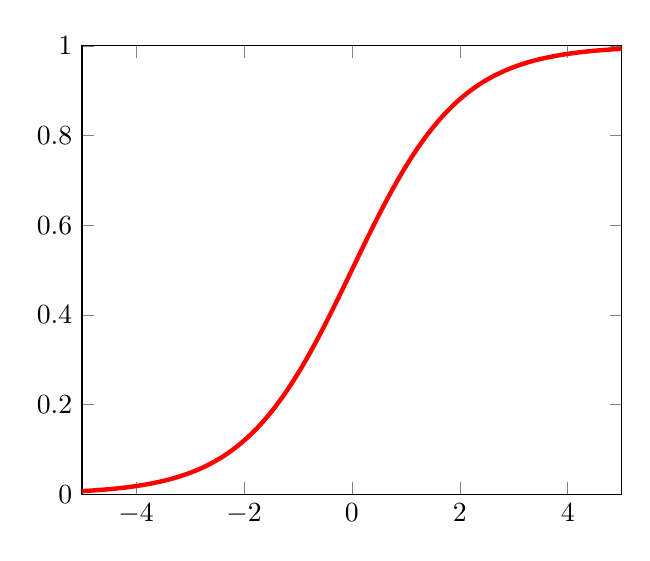
\begin{tikzpicture}
        \begin{axis}[xmin=-5, xmax=5, ymin=0, ymax=1, samples=150]
        \addplot[red, ultra thick] {1/(1+exp(-x))};
        \end{axis}
    \end{tikzpicture}
    
    }

\usetikzlibrary{positioning, calc}
\usetikzlibrary{arrows.meta}

\tikzstyle{circlebox}=[circle,thick,draw=black!75,minimum size=8mm]
\tikzstyle{inputnode}=[circlebox, draw=blue!75]
\tikzstyle{hiddennode}=[circlebox, draw=orange!75]
\tikzstyle{outputnode}=[circlebox, draw=orange!75]
\tikzstyle{simplebox}=[rectangle,thick,draw=black!75,
fill=black!20,minimum size=4mm]
\tikzstyle{textbox}=[rectangle,thick,minimum size=4mm,draw=black!0,
fill=black!0]
\tikzstyle{halfvdistance}=[yshift=-0.7cm]
\tikzstyle{abovebetween}=[xshift=-2.7mm]
\tikzstyle{edgepath} = [-Latex,->,shorten >=1pt,-stealth,semithick, rounded 
corners=5pt]

\def \nodedv {0.735cm}
\def \nodedh {0.65cm}

\tikzset{
    between/.style args={#1 and #2}{
        at = ($(#1)!0.5!(#2)$)
    }
}

\begin{document}
    \section{Subjects}
    \begin{itemize}
        \item Markov Decision Process
        \item Bellman Equations and Algorithms
    \end{itemize}
    
    \section{Notes}
    
    \subsection{Elements of reinforcement learning}

    \begin{description}
        \item[Exploration vs. exploitation] Should we explore new 
        opportunities, or take advantage of the ones we have found that works?
        \item[Agent] How do we interact with the environment, who do we 
        represent?
        \item[Environment] What actions can we take and what is currently 
        happening?
        \item[Policy] How does the learning agent behave? A mapping from the 
        perceived states of the environment to which actions to be taken when 
        in those states.
        \item[Reward signal] On each time step, the environment send the agent 
        a single number, a reward. The agents sole objective is to maximize the 
        total reward it receives. The agent can change the outcome by the 
        signal by taking actions or changing the environment, but can't change 
        the function that generates the reward signal.
        \item[Value function] The value of a state is the total amount of 
        reward an agent can expect to accumulate, \textit{starting from that 
        state}. Rewards return the immediate desirability of a state, value 
        returns the long-term desirability of a state.
        \item[Model of the environment] Something that mimics the behaviour of 
        the environment, so we can infer how the environment will behave. (E.g. 
        could be used to predict the next model). There are both model-based 
        and model-free methods.
    \end{description}
    
    \subsection{Finite Markov Decision Processes}
    We can think of the interaction between an agent and the environment as the 
    agent taking some action at time $t$ $A_t$, and the environment providing 
    the agent with a reward $R_{t+1}$ and a new state $S_{t+1}$ which prompts a 
    new action $A_{t+1}$ from the agent.
    
    At each time step $t$, the agent implements a mapping from states to 
    probabilities of selecting each possible action $A_t \in A(S_t)$. This 
    mapping is called the agent's policy and is denoted $\pi_t$ where 
    $\pi_t(a|s)$ is the probability that $A_t=a$ if $S_t=s$. Reinforcement 
    learning is about changing the policy as a result of experience.
    
    We seek to maximize the \textit{expected return} $\Ex({G_t})$, but how do 
    we define $G_t$? The simplest case is simply the sum of the rewards:
    
    \begin{equation*}
        G_t = R_{t+1}+R_{t+2}+\cdots+R_T
    \end{equation*}
    If we are dealing with \textit{episodic tasks}, i.e. tasks that are 
    independent like plays of a game or trips through a maze (we call these 
    tasks ``episodes''). However, if we 
    are dealing with \textit{continuing tasks}, for example a robot with a long 
    life span or process-control tasks then the return, which we are trying to 
    maximize is potentially infinite. Thus, we will use a definition of return 
    that is slightly more complex conceptually but much simpler mathematically. 
    We introduce the concept of \textit{discounting}, the agent will try to 
    maximize the sum of the discounted rewards, where the rewards are 
    decreasing in value so tasks that are performed immediately are worth more:
    \begin{equation*}
        G_t=R_{t+1}+\gamma R_{t+2}+ \gamma ^2 R_{t+3} + \cdots = 
        \sum_{k=0}^{\infty}\gamma^k R_{t+k+1}
    \end{equation*}
    Here $0\leq \gamma \leq 1$ is called the discount rate. Then we know that 
    if $\gamma < 1$ then the infinite sum has a finite value, as long as 
    $R_k\neq \infty$. If $\gamma = 0$, then the agent is only concerned with 
    maximizing immediate rewards. More often than not, we won't have $\infty$ 
    rewards, so we can simplify this to:
    \begin{equation*}
        G_t=\sum_{k=0}^{T-t-1}\gamma^k R_{t+k+1}
    \end{equation*}
    Where it is possible that $T=\infty$ or $\gamma = 1$ but both cannot be 
    true (since the sum would then be $\infty$).
    
    \subsubsection{The Markov Property}
    We cannot expect an actor to know everything about the environment, as some 
    information may be hidden. The environment will provide the actor with 
    different sensations, and we might expect the actor to remember all the 
    sensations it has experienced so far.
    
    We call a state signal which succeeds in retaining all relevant information 
    to be \textit{Markov} or to have \textit{the Markov property}. For example, 
    if we were playing chess, then the current configuration of all the pieces 
    on the board would serve as a Markov state, because it summarizes all 
    important details that led to it. Much of the information about the 
    sequence is lost, but all that really matters for the future of the game is 
    retained. It doesn't matter that we don't know how we ended up at that 
    chess board configuration, the current configuration is all that is 
    relevant.
    
    In order to formally define the Markov property in a mathematically simple 
    way, we will assume that there are a finit number of states and reward 
    values. This enables us to work in terms of sums and probabilities instead 
    of integrals and probability densities, but it can easily be extended.
    
    Consider how an environment might respond at time $t+1$ to the action taken 
    at time $t$. The most general, causal case is where the response depends on 
    everything that has happened earlier:
    \begin{equation*}
        \Pr\left[S_{t+1} =s', 
        R_{t+1}=r|S_0,A_0,R_1,S_1,A_1,\dots,R_{t-1},S_{t-1},A_{t-1},R_t,S_t,A_t 
         \right]
    \end{equation*}
    However, if the state signal has the Markov property, then the environments 
    response at $t+1$ only depends on the state and action at $t$ so we can 
    define it as simply:
    \begin{equation*}
        p(s',r|s,a)=\Pr\left[S_{t+1}=s',R_{t+1}=r|S_t=s, A_t=a\right]
    \end{equation*}
    If this hold for all $s'$ and $r$ then we will be able to predict the 
    result of an action having just $s$, $a$ just as good as we would be able 
    to do it given the complete history of states and actions.
    
    It is usually useful to think of the state at each time step as an 
    approximation to a Markov state even in non-Markov state signals because of 
    the better performance Markov gives us in reinforcement learning, as long 
    as one keeps in mind that it may not fully satisfy the Markov property.
    
    \subsubsection{Markov Decision Process}
    A reinforcement learning task that satisfies the Markov property is called 
    a \textit{Markov decision process} or MDP. If there is a finite amount of 
    states and actions, then we call it a \textit{finite MDP}. If you 
    understand \textit{finite MDP} then you understand $90\%$ of modern 
    reinforcement learning.
    
    A finite MDP, is defined by uts state and actions sets and by the one-step 
    dynamics of the environment. We use the probability of going to $s'$ and 
    receiving $r$ from $s$ and $a$ as previously:
    \begin{equation*}
    p(s',r|s,a)=\Pr\left[S_{t+1}=s',R_{t+1}=r|S_t=s, A_t=a\right]
    \end{equation*}
    This completely specify the dynamics of some finite MDP. We can then 
    compute anything else we might want to know about the environment such as 
    the expected rewards for state-action pairs:
    \begin{equation*}
        r(s,a)=\Ex\left[R_{t+1}|S_t=s, A_t=a\right]=\sum_{r\in R}r \sum_{s' \in 
        S} p(s',r|s,a)
    \end{equation*}
    The state-transition probabilities:
    \begin{equation*}
        p(s'|s,a)=\Pr\left[S_{t+1}=s'|S_t=s, A_t=a\right]=\sum_{r\in 
        R}p(s',r|s,a)
    \end{equation*}
    And the expected rewards for state--action--next-state:
    \begin{equation*}
        r(s,a,s')=\Ex\left[R_{t+1}|S_t=s,A_t=a,S_{t+1}=s'\right]=\frac{\sum_{r\in
         R}r\cdot p(s',r|s,a)}{p(s'|s,a)}
    \end{equation*}
    
    \subsubsection{Value Functions}
    We will need to estimate value functions for almost all reinforcement 
    learning algorithms. The value functions are functions of states that 
    estimate \textit{how good} it is to for the the agent to be in a given 
    state (or rather, how good is it to perform some action in a given state). 
    The notion of ``how good'' is defined in terms of what future rewards can 
    we expect to receive.
    
    A policy $\pi$ is a mapping from each state $s \in S$ and action $a \in 
    A(s)$ to the probability $\pi(a|s)$ of taking action $a$ when in state $s$. 
    Informally, the following equation is the expected return when starting in 
    state $s$ and following policy $\pi$ for a MDP:
    \begin{equation*}
        v_\pi(s)=\Ex_\pi\left[G_t\given
        S_t=s\right]=\Ex_\pi\left[\sum_{k=0}^{\infty}\gamma^k 
        R_{t+k+1}\given S_t=s\right]
    \end{equation*}
    
    Similarly, we can define the value of taking action $a$ in state $s$ under 
    $\pi$ as the expected return starting from $s$, taking the action $a$ and 
    then following $\pi$:
    \begin{equation*}
        q_\pi(s,a)=\Ex_\pi\left[G_t\given 
        S_t=s,A_t=a\right]=\Ex_\pi\left[\sum_{k=0}^{\infty}\gamma^kR_{t+k+1}\given
         S_t=s,A_t=a\right]
    \end{equation*}
    We call $q_\pi$ the action-value function for policy $\pi$. We can estimate 
    $v_\pi$ and $q_\pi$ using the average of the actual returns, we will return 
    to this later. For now, let's look at a fundamental property of $v_\pi$ 
    which is used throughout reinforcement learning. Namely, the property that 
    they satisfy particular recursive relationships:
    
    \begin{align*}
        v_\pi(s)&= \Ex_\pi\left[G_t\given S_t=s\right]\\
            &= \Ex_\pi\left[\sum_{k=0}^{\infty}\gamma^kR_{t+k+1}\given S_t = 
            s\right]\\
            &= 
            \Ex_\pi\left[R_{t+1}+\gamma\sum_{k=0}^{\infty}\gamma^kR_{t+k+2} 
            \given S_t=s\right]\\
            &= \sum_a \pi\left(a\given s\right) \sum_{s'} \sum_r p(s',r|s,a)
            \left[r+\gamma \Ex\left[\sum_{k=0}^{\infty}\gamma^k R_{t+k+2} 
            \given S_{t+1}=s'\right]\right]\\
            &= \sum_a \pi\left(a\given s\right) \sum_{s',r} p(s',r|s,a) 
            \left[r+\gamma v_\pi(s')\right]
    \end{align*}
    We can read this equation as a sum over the triples $a$, $s'$ and $r$. For 
    each triple, we compute its probability $\pi\left(a\given s\right)p(s', 
    r|s,a)$ weight the value in the bracket (which is the reward plus the 
    expected reward from the next state $s'$), which gives us the expected 
    value. This equation is called the \textit{Bellman equation for $v_\pi$}
    
    \subsubsection{Optimal value functions}
    In order to ``solve'' reinforcement learning, roughly means that we need to 
    find a policy that achieves a lot of reward in the long run. For finite 
    MDPs we can define it precisely as follows. A police $\pi$ is said to be 
    better than or equals to a policy $\pi'$ if its expected return is better 
    than or equal to that of $\pi'$. In other words $\pi \geq \pi' \iff 
    v_\pi(s)\geq v_{\pi'}(s) \forall s\in S$. There will always be at least one 
    policy which is better than or equal to all other policy which is the 
    optimal policy, we denote any of the optimal policies as $\pi_*$. We can 
    define their state-value function as:
    \begin{equation*}
        v_*(s)=\max_\pi v_\pi(s)
    \end{equation*}
    Which is the optimal state-value function. We can define the same for the 
    optimal action-value function:
    \begin{equation*}
        q_*(s,a)=\max_\pi q_\pi(s,a)
    \end{equation*}
    For the state-action pair $(s,a)$, this function gives the expected return 
    of taking action $a$ in state $s$ and then following an optimal policy. We 
    can therefore write $q_*$ in terms of $v_*$ as follows:
    \begin{equation*}
        q_*(s,a)=\Ex\left[R_{t+1}+\gamma v_*(S_{t+1}) \given S_t=s, A_t=a\right]
    \end{equation*}
    
    \subsubsection{Dynamic programming}
    We can use dynamic programmin (DP) to compute the value functions explained 
    earlier. Furthermore, we can easily obtain optimal policies once we have 
    found the optimal value functions $v_*$ or $q_*$ which satisfy the Bellman 
    equations:
    \begin{align*}
        v_*(s)&=\max_a \Ex\left[R_{t+1}+\gamma v_*(S_{t+1}) \given S_t=s, A_t = 
        a\right]\\
            &= \max_a \sum_{s',r}p(s',r|s,a)\left[r+\gamma v_*(s')\right]
    \end{align*}
    or
    \begin{align*}
        q_*(s,a) &= \Ex\left[R_{t+1}+\gamma \max_{a'}q_*(S_{t+1},a') \given 
        S_t=s, A_t=a \right]\\
            &= \sum_{s', r}p\left(s', r \given s,a\right)\left[r+\gamma 
            \max_{a'}q_*(s',a')\right]
    \end{align*}
    We will see that we obtain DP algorithms by turning these Bellman equations 
    into assigments, that is update rules which improve approximations of the 
    desired functions.
    
    \subsubsection{Policy Evaluation}
    First, we will consider computing the state-value function $v_\pi$. This is 
    called \textit{policy evaluation} recall that:
    \begin{align*}
    v_\pi(s) &= \Ex_\pi\left[\sum_{k=0}^{\infty}\gamma^kR_{t+k+1}\given S_t = 
    s\right]\\
        &= \Ex_\pi\left[R_{t+1}+\gamma v_\pi(S_{t+1}) 
        \given S_t=s\right]\\
        &= \sum_a \pi\left(a\given s\right) \sum_{s',r} p(s',r|s,a) 
        \left[r+\gamma v_\pi(s')\right]
    \end{align*}
    Now consider a sequence of approximate value functions $v_0,v_1,\dots$, the 
    initial approximation $v_0$ is arbitrary except the terminal state has to 
    be $0$. We can then obtain the approximations by using the Bellman equation 
    for $v_\pi$:
    \begin{align*}
        v_{k+1}(s)&= \Ex_\pi\left[R_{t+1}+\gamma v_k(S_{t+1}) \given S_t = s 
        \right]\\
            &=\sum_a \pi\left(a \given s\right)\sum_{s',r}p\left(s',r \given 
            s,a\right)\left[r+ \gamma v_k(s')\right]
    \end{align*}
    This approximation does indeed converge to $v_\pi$ as $k\rightarrow \infty$
    
    \subsubsection{Policy Improvement}
    Now that we are able to determine $v_\pi$, we are able to evaluate our 
    policies, and thus we will be able to improve upon them. For some state 
    $s$, we would like to know whether or not we should change the policy such 
    that we deterministically choose an action $a\neq \pi(s)$. We know the 
    quality of following the current policy from $s$ ($v_\pi(s)$), so would it 
    be better or worse to change to another policy? In order to answer this, we 
    could select $a$ in $s$ and otherwise just follow the existing policy:
    \begin{align*}
        q_\pi(s,a)&=\Ex\left[R_{t+1}+\gamma v_\pi(S_{t+1}) \given S_t=s, 
        A_t=a\right]\\
            &= \sum_{s',r}p\left(s',r \given s,a\right)\left[r+\gamma 
            v_\pi(s')\right]
    \end{align*}
    If this is greater than $v_\pi(s)$ then it is better to select $a$ once in 
    $s$, but then it would in fact be better to pick $s$ every time:
    \begin{equation*}
        q_\pi(s,\pi'(s)) \geq v_\pi(s) \implies v_{\pi'}(s) \geq v_\pi(s)
    \end{equation*}
    We can then use this to define a new greedy policy $\pi'$ given by:
    \begin{align*}
        \pi'(s)&=\arg\max_a q_\pi(s,a)\\
            &=\arg\max_a \Ex\left[R_{t+1} + \gamma v_\pi(S_{t+1}) \given S_t=s, 
            A_t=a \right]\\
            &=\arg\max_a \sum_{s',r}p\left(s',r \given s,a\right)\left[r+\gamma 
            v_\pi(s')\right]
    \end{align*}
    I.e. the greedy policy looks one step ahead and picks the action that looks 
    best in the short term. Now suppose $\pi'$ is as good as, but not better 
    than, the old policy $\pi$. The $v_\pi=v_{\pi'}$ and then it follows that:
    \begin{align*}
        v_{\pi'}(s)&=\max_a\Ex\left[R_{t+1}+\gamma v_{\pi'}(S_{t+1}) \given 
        S_t=s, A_t=a \right]\\
            &= \max_a \sum_{s',r}p\left(s',r \given s,a \right)\left[r+\gamma 
            v_{\pi'}(s')\right]
    \end{align*}
    But this was the optimal Bellman equation from earlier, therfore $v_{\pi'}$ 
    must be $v_*$ and thus $\pi'$ must be an optimal policy, thus this policy 
    improvement algorithm must give us a strictly better policy until we hit 
    the optimal one.
    
    So far, we have only considered deterministic policies, that is where 
    $\pi(s)$ always evaluate to the same action. However, all of the ideas so 
    far, easily extend to stochastic policies ($\pi(a|s)$).

    Now that we can both evaluate and improve our policies, we can just 
    continue evaluating then improving and evaluating then improve and so on, 
    monotonically improving untill we find a optimal solution.
    
    \subsubsection{Value iteration}
    This algorithm is fairly expensive, so we need to speed it up somehow. One 
    way is implementation specific, where we simply make sure to pick up policy 
    evaluation values from the last evaluation and not $0$.
    
    Value iteration provides us with a way to solve both policy evaluation and 
    improvement in one step.
    
    \begin{align*}
    v_{k+1}(s)&=\max_a\Ex\left[R_{t+1}+\gamma v_k(S_{t+1}) \given 
    S_t=s, A_t=a \right]\\
        &= \max_a \sum_{s',r}p\left(s',r \given s,a \right)\left[r+\gamma 
        v_k(s')\right]
    \end{align*}
    Here, we find that $v_k$ still converges to $v_*$.
    
    \subsubsection{Drawback of DP}
    The drawback of DP as described here, is that it involves operations over 
    the entire state set of the MDP, so if there are many states (like 
    backgammon) then it is incredibly expensive.
    
    \subsubsection{Generalized Policy Iteration}
    In generalized policy iteration (GPI), we maintain both an approximate 
    policy and an approximate value function. The value function is repeatedly 
    altered to approximate the value function for the current policy, and the 
    current policy is repeatedly improved with respect to the current value 
    function. In a way they move against each other, as they create a moving 
    target for each other, but they cause both policy and value function to 
    approach optimality.
    
    This is a simple overview of the generalized policy iteration:
    \begin{itemize}
        \item While improving repeat
        \item Run policy evaluation for some time on some states
        \item Run policy improvement for som time on some states
    \end{itemize}
    Here we may choose not to visit all states, but in most cases we will still 
    converge in polynomial time.
    
    \subsection{Monte Carlo algorithms}
    Up until now, we have assumed complete knowledge of the environment (finite 
    states and actions). Monte Carlo algorithms, allows us to learn from just 
    \textit{experience} -- we cample sequences of states, action and rewards 
    without any prior knowledge of the environment's dynamics.
    
    In the Monte Carlo methods, we want to sovle the reinforcement learning 
    problem based on averaging sample returns. Furthermore instead of computing 
    the value functions (as we did in DP), we here want to learn the value 
    functions instead.
    
    What if we looked at just the state-value function, how would we try to 
    estimate that? The obvious solution here, is to average all the returns 
    observed after visits to that state. As we observe more and more returns, 
    the average should converge to the expected value. This is the underlying 
    idea of all Monte Carlo algorithms.
    
    In order to ensure well-defined returns are available, we will only 
    consider Monte Carlo for episodic tasks.
    
    \subsubsection{Estimating $v_\pi(s)$}
    $v_\pi(s)$ is the value of a state $s$ under policy $\pi$, given a set of 
    episodes obtained by following $\pi$ and passing through $s$. Each 
    occurrence of state $s$ in an episode is called a \textit{visit} to $s$. It 
    may happen that we visit $s$ multiple times in an episode, so we will look 
    at the \textit{first visit} to $s$. Let's first look at a theoretical 
    algorithm which computes the value of $s$ in the first visit to $s$:
    \begin{algorithm}
        \caption{First-visit MC policy evaluation}
        \begin{algorithmic}
            \State \textit{// Initialize:}
            \State $\pi \gets$ policy to be evaluated
            \State $V \gets $ an arbitrary state-value function
            \State $Returns(s) \gets $ an empty list, for all $s \in S$
            \State
            \Loop \, forever
                \State Generate an episode using $\pi$
                \ForAll{state $s$ in the episode}
                    \State $G \gets $ return following the first occurence of 
                    $s$
                    \State Append $G$ to $Returns(s)$
                    \State $V(s) \gets \average(Returns(s))$
                \EndFor
            \EndLoop
        \end{algorithmic}
    \end{algorithm}
    
    We could also have explored the \textit{every-visit MC method}, which has 
    some different properties and extends more naturally to function 
    approximation, but First-visit MC has been more widely studied.
    
    First-visit MC converges quadratically to $v_\pi(s)$ as the number of 
    first-visits to $s$ 
    goes to infinity. An alternative, finite option, is to loop for some time 
    or some number of episodes.
    
    \subsubsection{Estimation of action values}
    If a model is available, we can simply look ahead in the next possible 
    states and pick the action that leads to the best state. If no model is 
    available, then we have to estimate the values of the action (e.g. speed of 
    vehicle) we should pick in order to get to the best state and maximize 
    reward.
    
    In other words, one of the primary goals for Monte Carlo methods is to 
    estimate $q_*$, which is the optimal value we get when we take action $a$ 
    from state $s$. In order to estimate this, we may run a First-visit MC 
    method as before, just visiting state-action pairs instead of just states. 
    Again, this will converge quadratically as before.
    
    The complication is that many state-action pairs may never be visited. If 
    $\pi$ is a deterministic policy, then following $\pi$ one will only observe 
    returns from one action from each state (as it is deterministic). Therefore 
    the Monte Carlo estimates of the other actions from that state will not 
    improve with experience. This is the general problem of \textit{maintaining 
    exploration} i.e. we must assure that we are continually exploring other 
    options in order to attempt to find a better one. One way to solve this, is 
    to say that we start in a state-action pair, and every state-action pair 
    has a nonzero probability of being selected as the start. We call this the 
    assumption of \textit{exploring starts}.
    
    \textit{Exploring starts}, is not really useful when we learn by actual 
    interacting with an environment as we cannot simply start from any state we 
    want. In this case, the most common alternative approach is to only 
    considering stochastic policies with only nonzero probabilities.
    
    \subsubsection{Approximating optimal policies}
    Let us consider a Monte Carlo version of classical policy iteration. We can 
    perform policy evaluation as described in the previous section (estimation 
    of action values). If we assume that:
    \begin{itemize}
        \item We observe an infinite number of episodes.
        \item The episodes are generated with exploring starts.
    \end{itemize}
    Then the Monte Carlo methods will compute each $q_{\pi_k}$ exactly for 
    arbitrary $\pi_k$.
    
    Now we just need to figure out how to perform policy-improvements. We can 
    improve on our policy with a simple greed policy with respect to the 
    current value function. We can then compute for each $s \in S$ the policy 
    $\pi$:
    \begin{equation*}
        \pi(s) = \arg\max_a q(s,a)
    \end{equation*}
    We can then construct each $\pi_{k+1}$ as the greedy policy with respect to 
    $q_{\pi_k}$, and we get that the policy improvement theorem applies since:
    \begin{align*}
        q_{\pi_k}(s,\pi_{k+1}(s)) &= q_{\pi_k}(s, \arg\max_a q_{\pi_k}(s,a))
    \end{align*}
    This assures us that each $\pi_{k+1}$ is uniformly better than or just as 
    good as $\pi_k$. If it is just as good as $\pi_k$ then they are both 
    optimal policies.
    
    \subsubsection{Monte Carlo without infinite episodes}
    We made two unlikely assumptions in order to easily obtain this guarantee 
    of convergence. One was that the episodes has exploring starts, the other 
    was that we could run for infinitely many episodes. We will try to remove 
    the latter assumption here and then return to exploring starts afterwards.
   
    There are two primary ways to combat the infinite episodes assumption, one 
    approach is to estimate some bounds on magnitude and probability of error 
    and run until these bounds are sufficiently small. This will guarantee 
    correct convergence up to some level of approximation, however it is likely 
    to require far too many episodes to be useful in practice.
    
    The second approach is to avoid trying to complete policy evaluation before 
    returning for improvement and simply move the value function \textit{toward}
    $q_{\pi_k}$. One extreme example of this was the value iteration, in which 
    only one iteration of iterative policy evaluation is performed between 
    improvements. Or the in-place version where we alternate between 
    improvement and evaluation steps for single states.
    
    For Monte Carlo policy evaluation it is natural to alternate between 
    evaluation and improvement on an episode-by-episode basis. After each 
    episode we evaluate the policy and then improve it at all the visited 
    states. We can describe this algorithm as follows:
    
    \begin{algorithm}
        \caption{Monte Carlo ES (Exploring Starts)}
        \begin{algorithmic}
            \State \textit{// Initialize, for all } $s\in S, a\in A(s)$:
            \State $Q(s,a) \gets$ arbitrary
            \State $\pi(s) \gets$ arbitrary
            \State $Returns(s,a) \gets$ empty list
            \State
            \Loop\, forever
                \State Choose $S_0 \in S$ and $A_0 \in A(S_0)$ s.t. all pairs 
                have probability $> 0$
                \State Generate an episode starting from $S_0, A_0$ following 
                $\pi$
                \ForAll{pairs $s,a$ appearing in the episode}
                    \State $G \gets$ return following the first occurence of 
                    $s,a$
                    \State Append $G$ to $Returns(s,a)$
                    \State $Q(s,a) \gets \average(Returns(s,a))$
                \EndFor
                \ForAll{states $s$ in the episode}
                    \State $\pi(s) \gets \arg \max_a Q(s,a)$
                \EndFor
            \EndLoop
        \end{algorithmic}
    \end{algorithm}
    
    \subsubsection{Monte Carlo without Exploring Starts}
    Now, how can we avoid the unlikely assumption of exploring starts? The only 
    general way to ensure that all actions are selected infinitely often is for 
    the agent to continue to select them. We have two approaches to ensuring 
    that this happens, we call it \textit{on-policy} methods  and 
    \textit{off-policy} methods. On-policy attempts to evaluate or improve the 
    policy used to make decision whereas off-policy methods evaluate or improve 
    a different policy. The ES method above is an example of an on-policy 
    method. We will explore on-policy methods more here, and not go into 
    details with off-policy.
    
    Here we will look at $\epsilon$-greedy policies, which with probability 
    $1-\epsilon$ will simply follow the policy $\pi$, but with probability 
    $\epsilon$ it will select a uniformly random action. So each action has 
    probability $\frac{\epsilon}{|A(s)|}$ of being picked, except the estimated 
    optimal action which also has probability $1-\epsilon$ of being picked, 
    yielding the algorithm:
    
    \begin{algorithm}
        \caption{On-policy first-visit MC control (for $\epsilon$-soft 
        policies)}
        \begin{algorithmic}
            \State \textit{// Initialize}
            \ForAll{$s \in S$ and $a \in A(s)$}
                \State $Q(s,a) \gets$ arbitrary
                \State $Returns(s,a) \gets$ empty list
                \State $\pi(a|s) \gets$ an arbitrary $\epsilon$-soft policy
            \EndFor
            
            \Loop\, forever
                \State Generate an episode using $\pi$
                \ForAll{pairs $s,a$ appearing in the episode}
                    \State $G \gets$ return following the first occurence of 
                    $s,a$
                    \State Append $G$ to $Returns(s,a)$
                    \State $Q(s,a) \gets \average(Returns(s,a))$
                \EndFor
                \ForAll{visited states $s$ in the episode}
                    \State $A^* \gets \arg\max_a Q(s,a)$
                    \ForAll{$a \in A(s)$}
                        \State $\pi(a|s) \gets \begin{cases}
                        1-\epsilon + \frac{\epsilon}{|A(s)|},&\text{ if 
                        }a=A^*\\
                        \frac{\epsilon}{|A(s)|},&\text{ if } a \neq A^*
                        \end{cases}$
                    \EndFor
                \EndFor
            \EndLoop
        \end{algorithmic}
    \end{algorithm}
    
    This holds under the policy improvement theorem, although I will not prove 
    this here.
\end{document}